
In the last three Chapters we have introduced six important \PETSc types (object classes).  All are important for solving PDEs:
\begin{itemize}
\item[\quad Chapter \ref{chap:ls}:] \pVec, \pMat, \pKSP, \pPC
\item[\quad Chapter \ref{chap:st}:] \pDMDA
\item[\quad Chapter \ref{chap:nl}:] \pSNES
\end{itemize}

Each example in the rest of the book will use \emph{all} of these types.  From now on we will even solve linear PDEs using a \pSNES object.  Linear problems are now merely the case where we know that one Newton iteration suffices in theory.  Always using \pSNES gives us uniform code structure and much more flexibility when it comes to changing the PDE problem.

Though new ideas appear in it, the current Chapter takes a break from introducing new \PETSc types.  Instead we look at a PDE which arises from minimization in a function space, and introduce a structured-grid finite element method.  Our one example is a nonlinear PDE which is Poisson-like, but with solution-dependent diffusivity.

Also, the example code in this Chapter is shown in full, but it is that last one shown like that.  In later Chapters we show snippets of example codes, assuming the reader can examine the complete codes in the \texttt{p4pdes} repository; see Chapter \ref{chap:gs}.


\section{$p$-Laplacian equation as minimization}

Let $\Omega$ be a domain (connected open subset) in $\RR^2$ or $\RR^3$ with well-behaved boundary.\sidenote{A Lipschitz boundary will suffice in theory.  In practice we use polygonal domains, namely a rectangle in the current Chapter and general polygons in Chapter \ref{chap:un}.}  For simplicity, because our numerical method will use the point values of this given function, assume we have chosen $f\in C(\Omega)$.  Consider this functional for $p \ge 1$,
\begin{equation}
    I[u] = \int_\Omega \frac{1}{p} |\grad u|^p - fu.  \label{eq:of:functional}
\end{equation}

The nonlinear functional $I[u]$ is well-defined on the Sobolev space \citep{AdamsFournier2003,Evans2010} of integrable functions on $\Omega$ which have integrable gradient,
\begin{equation}
    W^{1,p}(\Omega) = \left\{w \,:\, \int_\Omega |w|^p < \infty \,\, \& \, \int_\Omega |\grad w|^p < \infty\right\}. \label{eq:of:sobolevdefn}
\end{equation}
This is a Banach space with norm $\|w\|_{W^{1,p}} = \left(\int_\Omega |w|^p + \int_\Omega |\grad w|^p\right)^{1/p}$.

\begin{marginfigure}
\includegraphics[width=1.2\textwidth]{figs/minsurf} % generated by figs/minsurf.tex
\medskip
\caption{The functional $I[u]$ is analogous to the convex surface $z = \tfrac{1}{4}(x^4 + y^4) - 2x + 2y$ shown here, but with input from the $\infty$-dimensional space $W_g^{1,p}(\Omega)$ instead of the plane $\RR^2$.}
\label{fig:of:cartoonfunctional}
\end{marginfigure}

The reader may visualize $I[u]$ in cartoon form as in Figure \ref{fig:of:cartoonfunctional}.  As suggested by the cartoon, this functional has a unique minimum, at least once we add boundary conditions.  We add Dirichlet conditions (Chapter \ref{chap:st}) by choosing a real-valued function $g$, defined along $\partial \Omega$, so as to determine an affine subspace of $W^{1,p}(\Omega)$, namely
\begin{equation}
    W_g^{1,p}(\Omega) = \left\{w \,:\, w \in W^{1,p}(\Omega) \,\, \& \,\, w\big|_{\partial \Omega} = g\right\}.  \label{eq:of:affinedirichlet}
\end{equation}
For this to make sense one might require $g \in L^p(\partial \Omega)$ and note that the equation $w\big|_{\partial \Omega} = g$ has a precise ``trace operator'' meaning \citep[section 5.5]{Evans2010}.  Again, however, because our numerical scheme will use the point values of $g$, we assume $g\in C(\partial\Omega)$.

The above considerations also define the vector subspace $W_0^{1,p}(\Omega) \subset W^{1,p}(\Omega)$ in the case where $g=0$.  We will use this subspace for ``test functions'' below.

The functional $I[u]$ has two significant properties.  First, with the boundary conditions, $I[u]$ is \emph{coercive} in the sense that if the input function from $W_g^{1,p}(\Omega)$ is large in norm then the output is large:
\begin{equation}
\lim_{\|u\|_{W^{1,p}} \to +\infty} I[u] = +\infty.   \label{eq:of:coercivity}
\end{equation}
Second it is \emph{convex}, meaning that
\begin{equation}
I[\lambda u + (1-\lambda) v] \le \lambda I[u] + (1-\lambda) I[v]    \label{eq:of:convexity}
\end{equation}
if $u,v\in W_g^{1,p}(\Omega)$ and $0 \le \lambda \le 1$.  (We say inequality \eqref{eq:of:convexity} is \emph{strict} if $\|u-v\|_{W^{1,p}} > 0$ and $0 < \lambda < 1$.)
These two properties of $I[u]$, coercivity and convexity, are addressed in Exercise \ref{chap:of}.\ref{exer:of:twoproperties}.

A standard theorem in the calculus of variations \citep[Theorem 8.2.2]{Evans2010} shows that the coercivity and strict convexity of $I[u]$ imply that the problem
\begin{equation}
\min_{u \in W_g^{1,p}(\Omega)} I[u] \label{eq:of:plapmin}
\end{equation}
has a unique solution.  Strict convexity is used to show uniqueness, but convexity also implies that $I[u]$ is continuous enough to have a minimum on compact sets in the appropriate topology.\sidenote{Namely $I[u]$ is \emph{weakly lower semi-continuous}. This means, by definition, that $\liminf_{v\rightharpoonup u} I[v] \ge I[u]$, using the weak topology on $W^{1,p}(\Omega)$ \citep[section 8.2]{Evans2010}.}  Compactness arises from coercivity in the sense that bounded, closed subsets of $W^{1,p}(\Omega)$, which arise in the existence proof as sets $\{w\,:\,I[w] \le L\}$, are compact in the weak topology.

Being good calculus students we seek the solution to minimization problem \eqref{eq:of:plapmin} by taking the derivative and setting it to zero.  Fortunately, if $p>1$ then the functional $I[u]$ is smooth enough to have a gradient, as we show next.  The solution of minimization \eqref{eq:of:plapmin} is then also the solution to a nonlinear equation.  It has several names, including \emph{variational equation}, \emph{Euler-Lagrange equation}, and the \emph{weak form of the PDE}.

Assume $\eps\in \RR$ and $u,v \in W^{1,p}(\Omega)$.  Then, by the binomial theorem,
\begin{align*}
I[u+\eps v] - I[u] &= \int_\Omega \frac{1}{p} |\grad u + \eps \grad v|^p - \frac{1}{p} |\grad u|^p - \eps f v \\
   &= \eps \left(\int_\Omega |\grad u|^{p-2} \grad u \cdot \grad v - f v\right) + O(\eps^2).
\end{align*}
Thus the directional derivative exists and has this formula:
\begin{equation}
\grad I[u](v) = \lim_{\eps\to 0} \frac{I[u+\eps v] - I[u]}{\eps} = \int_\Omega |\grad u|^{p-2} \grad u \cdot \grad v - f v. \label{eq:of:plapfunctionalderivative}
\end{equation}
That is, for each $u \in W^{1,p}(\Omega)$, formula \eqref{eq:of:plapfunctionalderivative} defines a linear and continuous map, the gradient
   $$\grad I[u] : W^{1,p}(\Omega) \to \RR.$$

If $u \in W_g^{1,p}(\Omega)$ and $v\in W_0^{1,p}(\Omega)$ then $u+\eps v\in W_g^{1,p}(\Omega)$.  Thus if $u \in W_g^{1,p}(\Omega)$ solves \eqref{eq:of:plapmin} then the above calculation also shows $\grad I[u](v)=0$ or
\begin{equation}
\int_\Omega |\grad u|^{p-2} \grad u \cdot \grad v - f v = 0 \label{eq:of:plapweakform}
\end{equation}
for all $v\in W_0^{1,p}(\Omega)$.  Note that the test functions $v$ have zero boundary values in this calculation.  We refer to \eqref{eq:of:plapweakform} as the \emph{weak form} of the $p$-\emph{Laplacian} equation.

If the solution $u \in W_g^{1,p}(\Omega)$ to minimization problem \eqref{eq:of:plapmin} or equation \eqref{eq:of:plapweakform} is actually smooth enough to have continuous second derivatives\sidenote{\emph{Proving} this much smoothness is possible in some cases when the domain $\Omega$ and data $f,g$ are well-behaved, but beyond our scope.} then we can derive the \emph{strong form} PDE as follows.  An integration-by-parts \citep[Appendix C]{Evans2010} gives
    $$-\int_\Omega \Div\left(|\grad u|^{p-2} \grad u\right) v - \int_\Omega f v + \int_{\partial \Omega} v |\grad u|^{p-2} \grad u \cdot \bn = 0.$$
The boundary integral is zero because $v\in W_0^{1,p}(\Omega)$.  It follows that
\begin{equation}
- \Div\left(|\grad u|^{p-2} \grad u\right) = f.
\label{eq:of:plapstrongform}
\end{equation}
This strong form is the traditional form of the $p$-Laplacian equation.  It reduces to the Poisson equation \eqref{poissonsquare} if $p=2$.

Before proceeding to a numerical solution, the main ideas of the above diversion into theory are simple and thus worth restating:
\begin{quote}
Minimization problem \eqref{eq:of:plapmin} for functional $I[u]$ in \eqref{eq:of:functional} is equivalent to the weak form \eqref{eq:of:plapweakform}.  It becomes the strong form \eqref{eq:of:plapstrongform} in cases where the solution $u$ is smooth.  Thus the $p$-Laplacian equation, in either form \eqref{eq:of:plapweakform} or \eqref{eq:of:plapstrongform}, arises from minimization.
\end{quote}


\section{Structured $Q^1$ finite elements}

We can use \PETSc to numerically solve the $p$-Laplacian equation as minimization problem \eqref{eq:of:plapmin}, based only on user code that computes the functional $I[u]$ from a representation of $u \in W_g^{1,p}(\Omega)$.  Thus, once we have a finite-dimensional representation of the input $u$, all we need to implement is formula \eqref{eq:of:functional} for $I[u]$.

Such a minimization approach may suffice for initial prototyping.  It can then be augmented by additional derivative-computing code, as we show, in which case the problem becomes a nonlinear-residual problem like that of Chapter \ref{chap:nl}.  Initially, however, we will ask \PETSc to use finite differences when it needs derivatives (gradients) in minimizing $I[u]$.  In this case the system of nonlinear equations, with associated residual function, is internal to \PETSc, and only approximate.

For the representation of $u$ we introduce a structured-grid finite element method (FEM) using quadrilateral elements.  The gridded unknowns, which live on the same structured grid as in Chapter \ref{chap:st}, now represent a function in a function space.  The resulting code will be similar to a finite difference solution of PDE \eqref{eq:of:plapstrongform}, despite the conceptual changes.

\begin{marginfigure}
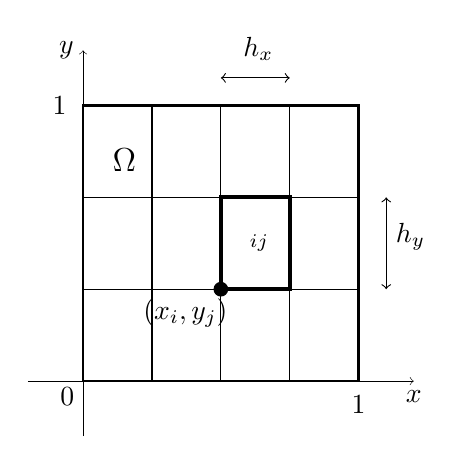
\begin{tikzpicture}[scale=3.5]
  \draw[->,very thin] (-0.2,0.0) -- (1.2,0.0) node[below] {$x$};
  \draw[->,very thin] (0.0,-0.2) -- (0.0,1.2) node[left] {$y$};
  \draw[line width=1.0pt] (0.0,0.0) -- (0.0,1.0) -- (1.0,1.0) -- (1.0,0.0) -- cycle;
  \pgfmathsetmacro\fourth{1.0/4.0}
  \pgfmathsetmacro\third{1.0/3.0}
  \pgfmathsetmacro\twothird{2.0/3.0}
  \draw[xstep=\fourth,ystep=\third,black,thin] (0.0,0.0) grid (1.0,1.0);
  % outline an element
  \draw[line width=1.5pt] (0.5,\third) -- (0.75,\third) -- (0.75,\twothird) -- (0.5,\twothird) -- cycle;
  \node at (0.64,0.5) {$\square_{ij}$};
  \filldraw (0.5,\third) circle (0.7pt) node[xshift=-4.5mm,yshift=-3mm] {$(x_i,y_j)$};
  \draw[<->] (0.5,1.1) -- (0.75,1.1) node[above,yshift=1mm,xshift=-4mm] {$h_x$};
  \draw[<->] (1.1,\third) -- (1.1,\twothird) node[right,yshift=-5mm] {$h_y$};
  \node at (0.15,0.8) {\large $\Omega$};
  \node[yshift=-3mm] at (1.0,0.0) {$1$};
  \node[xshift=-3mm] at (0.0,1.0) {$1$};
  \node[xshift=-2mm,yshift=-2mm] at (0.0,0.0) {$0$};
\end{tikzpicture}
\caption{Our domain $\Omega$ is a unit square.  The structured grid divides it into elements $\square_{ij}$ of area $h_x h_y$ indexed by their lower-left corners $(x_i,y_j)$.}
\label{fig:of:q1grid}
\end{marginfigure}

The domain is fixed to be the square $\Omega = (0,1)\times (0,1)$.  Consider the structured grid on $\Omega$ shown in Figure \ref{fig:of:q1grid}.  For positive integers $m_x$ and $m_y$ let $h_x=1/(m_x-1)$ and $h_y=1/(m_y-1)$.  The grid has nodes $(x_i,y_j)$ where $x_i = i h_x$ and $y_j = j h_y$, for indices $0\le i \le m_x-1$ and $0 \le j \le m_y-1$.  The \emph{elements} are the (closed) rectangles
   $$\square_{ij} = [x_i,x_{i+1}] \times [y_j,y_{j+1}].$$
Observe that $\bigcup_{ij} \square_{ij} = \overline{\Omega}$ and $|\square_{ij}| = h_x h_y$.

We immediately see that the functional in \eqref{eq:of:functional} can be computed element-by-element, because the element boundaries are of zero measure and integration is additive:
\begin{equation}
I[u] = \sum_{i=0}^{m_x-1} \sum_{j=0}^{m_y-1} \int_{\square_{ij}} \frac{1}{p} |\grad u|^p - fu  \label{eq:of:sumoverelements}
\end{equation}
Integration over a single element $\square_{ij}$ can be addressed once we represent $f$ and $u$.  A very similar sum over elements computes an approximation of the weak form \eqref{eq:of:plapweakform}.

So, how should we approximate a function $w \in W^{1,p}(\Omega)$ in a manner compatible with the structured grid of rectangles above?  One of the simpler choices is to require that the approximation $w_h \approx w$ be bilinear on each element $\square_{ij}$ and continuous on the whole domain $\Omega$.  These requirements allow us to determine $w_h(x,y)$, for any $(x,y)\in \overline\Omega$, from the nodal values $w_{ij} = w_h(x_i,y_j)$.  Said another way, there is a linear isomorphism between the vector space $\RR^N$ of possible nodal values, with $N=m_x m_y$ equal to the total number of nodes, and an $N$-dimensional linear subspace of $W^{1,p}(\Omega)$, namely
\begin{equation}
S^h = \left\{v \in C(\Omega) \, \Big| \, v|_{\square_{ij}} \text{ is bilinear}\right\}. \label{eq:of:Shdefn}
\end{equation}
Because the elements are quadrilaterals and the degree of bilinear polynomials is one, $S^h$ is a $Q^1$ \emph{finite element space} \citep{Elmanetal2005}

The solution $u$ to minimization problem \eqref{eq:of:plapmin} must, however, have the boundary values given by $g$.  If $g$ is discontinuous or not piecewise-linear then its use as boundary values conflicts with the restrictions which define $S^hh$.  We resolve the conflict by requiring $g$ to be well-behaved, namely continuous and (appropriately) piece-wise linear on $\partial\Omega$.  One may show in that case that the (affine) space of functions
\begin{equation}
S_g^h = \left\{v \in S^h \, \Big| \, v|_{\partial \Omega} = g\right\} \label{eq:of:Sghdefn}
\end{equation}
is an (affine) subspace of $W_g^{1,p}(\Omega)$.  Replacing $W_g^{1,p}(\Omega)$ by $S_g^h$ in problem \eqref{eq:of:plapmin} gives a \emph{conforming}\sidenote{A ``nonconforming'' version might only have $u_h \approx g$ on the boundary.  For example, $u_h|_{\partial \Omega}$ might be a piecewise-linear interpolant of $g$.} $Q^1$ FEM in which the FEM solution $u_h\in S_g^h$ is also in $W_g^{1,p}(\Omega)$.

The next step is to describe a bilinear function on a single element $\square_{ij}$, and to thereby build a basis for space $S_g^h$.  We do this by constructing bilinear functions on a \emph{reference element}
    $$\square_\ast = [-1,1]\times[-1,1],$$
in variables $\xi$ and $\eta$, as shown in Figure \ref{fig:of:q1gridandref}.\sidenote{One can avoid the reference element in the case here, in which all elements in the structured grid are congruent rectangles \citep[for example]{Bueler2015}.  However, we are thinking ahead toward less-structured examples (Chapter \ref{chap:un}).}

If $v(\xi,\eta)$ is bilinear on $\square_\ast$ then $v(\xi,\eta) = a + b\, \xi + c\, \eta + d\, \xi \eta$.  The monomial basis $\{1,\xi,\eta,\xi\eta\}$ is not, however, a convenient one.  Instead, number the vertices (nodes) of $\square_\ast$ as shown in Figure \ref{fig:of:q1gridandref}:
\begin{align}
(\xi_0,\eta_0) &= (-1,-1), \quad (\xi_1,\eta_1) = (+1,-1),    \label{eq:of:refcorners} \\
(\xi_2,\eta_2) &= (+1,+1), \quad (\xi_3,\eta_3) = (-1,+1). \notag
\end{align}
The four functions
\begin{equation}
\chi_\ell(\xi,\eta) = \frac{1}{4} \left(1 + \xi_\ell \xi\right) \left(1 + \eta_\ell \eta\right)  \quad \text{ for } \ell=0,1,2,3 \label{eq:of:chidefn}
\end{equation}
form a basis of bilinear functions on $\square_\ast$ so that
    $$\chi_\ell(\xi_{\ell'},\eta_{\ell'}) = \delta_{\ell\ell'}.$$
Expanding in this basis is easy because
\begin{equation}
v(\xi,\eta) = \sum_{\ell=0}^3 v_\ell \chi_\ell(\xi,\eta) \label{eq:of:bilinearrepresentationref}
\end{equation}
where $v_\ell = v(\xi_\ell,\eta_\ell)$; the coefficients are the nodal values.

\begin{figure}
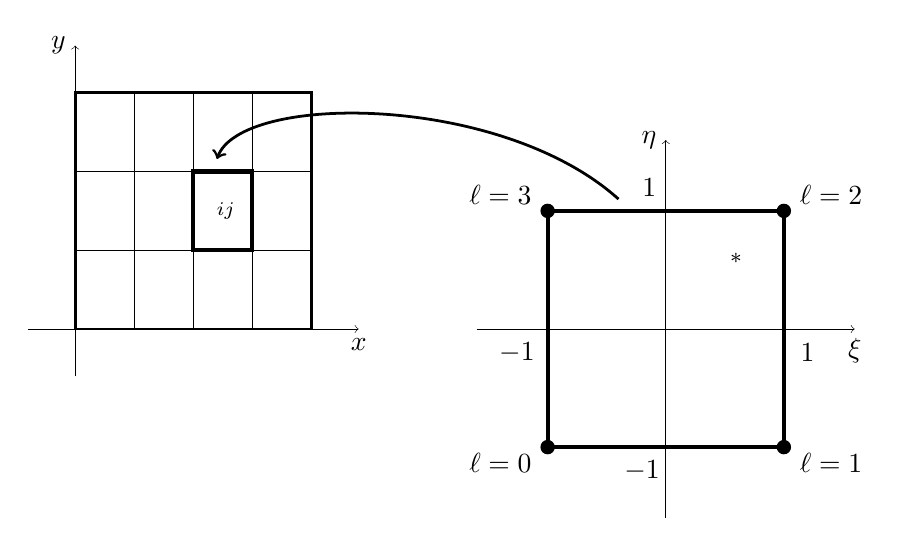
\begin{tikzpicture}[scale=3.0]
% (x,y) elements
  \draw[->,very thin] (-0.2,0.0) -- (1.2,0.0) node[below] {$x$};
  \draw[->,very thin] (0.0,-0.2) -- (0.0,1.2) node[left] {$y$};
  \draw[line width=1.0pt] (0.0,0.0) -- (0.0,1.0) -- (1.0,1.0) -- (1.0,0.0) -- cycle;
  \pgfmathsetmacro\fourth{1.0/4.0}
  \pgfmathsetmacro\third{1.0/3.0}
  \pgfmathsetmacro\twothird{2.0/3.0}
  \draw[xstep=\fourth,ystep=\third,black,thin] (0.0,0.0) grid (1.0,1.0);
  % outline an element
  \draw[line width=1.5pt] (0.5,\third) -- (0.75,\third) -- (0.75,\twothird) -- (0.5,\twothird) -- cycle;
  \node at (0.64,0.5) {$\square_{ij}$};

% (xi,eta) reference element
% origin of axes at (2.5,0.0) and square has half-width 0.5
  \draw[->,very thin] (1.7,0.0) -- (3.3,0.0) node[below] {$\xi$};
  \draw[->,very thin] (2.5,-0.8) -- (2.5,0.8) node[left] {$\eta$};
  \draw[line width=1.5pt] (2.0,-0.5) -- (3.0,-0.5) -- (3.0,0.5) -- (2.0,0.5) -- cycle;
  \node at (3.1,-0.1) {$1$};
  \node at (1.87,-0.1) {$-1$};
  \node at (2.43,0.6) {$1$};
  \node at (2.4,-0.6) {$-1$};
  \node at (2.8,0.3) {\large $\square_\ast$};
  \filldraw (2.0,-0.5) circle (0.8pt) node[xshift=-6mm,yshift=-2mm] {$\ell=0$};
  \filldraw (3.0,-0.5) circle (0.8pt) node[xshift=6mm,yshift=-2mm] {$\ell=1$};
  \filldraw (3.0,0.5) circle (0.8pt) node[xshift=6mm,yshift=2mm] {$\ell=2$};
  \filldraw (2.0,0.5) circle (0.8pt) node[xshift=-6mm,yshift=2mm] {$\ell=3$};

% arc
  \draw[->,line width=1.0pt] (2.3,0.55) .. controls (1.8,1.0) and (0.7,1.0) .. (0.6,0.72);
\end{tikzpicture}
\caption{Each element $\square_{ij}$ is the image under a map from the reference element $\square_\ast$.  The corners of $\square_\ast$ are numbered $\ell=0,1,2,3$.}
\label{fig:of:q1gridandref}
\end{figure}

The element map $\square_\ast \to \square_{ij}$ pictured in Figure \ref{fig:of:q1gridandref} can be written using the above basis functions\sidenote{This form applies even in the case of logically-structured grids of quadrilaterals which are deformed in the $(x,y)$ plane, so-called \emph{isoparametric} finite elements \citep{Elmanetal2005}.} $\chi_\ell$, but then one can simplify significantly:
\begin{align}
x(\xi,\eta) &= \sum_{\ell=0}^3 x_\ell \chi_\ell(\xi,\eta) = x_i + \frac{h_x}{2} (1+\xi), \label{eq:of:referencemap} \\
y(\xi,\eta) &= \sum_{\ell=0}^3 y_\ell \chi_\ell(\xi,\eta) = y_j + \frac{h_y}{2} (1+\eta). \notag
\end{align}
The Jacobian of this map, used in integrals below, is the ratio of the area of $\square_{ij}$ to the area of $\square_\ast$:
\begin{equation}
\det\frac{\partial(x,y)}{\partial(\xi,\eta)} = \det\begin{bmatrix} \frac{h_x}{2} & 0 \\ 0 & \frac{h_y}{2} \end{bmatrix} = \frac{h_x h_y}{4}. \label{eq:of:elementjacobian}
\end{equation}

\begin{marginfigure}
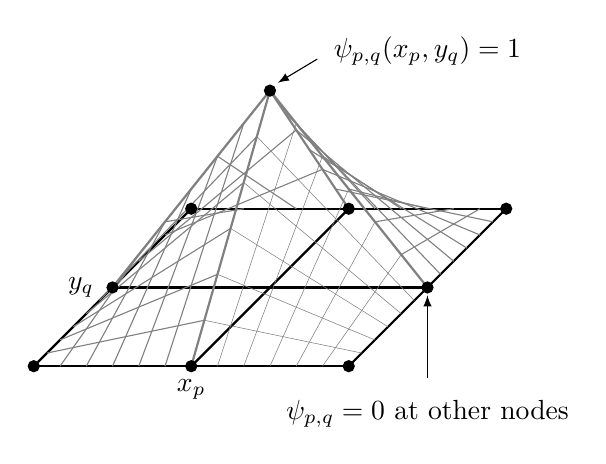
\begin{tikzpicture}[scale=0.5]

  % strong grid around elements
  \draw[thick] (0,0) -- (8,0);
  \draw[thick] (2,2) -- (10,2);
  \draw[thick] (4,4) -- (12,4);
  \draw[thick] (0,0) -- (4,4);
  \draw[thick] (4,0) -- (8,4);
  \draw[thick] (8,0) -- (12,4);

  \def\ytop{7};

  % tent lines
  \draw[gray,thick] (6,\ytop) -- (4,0);
  \draw[gray,thick] (6,\ytop) -- (2,2);
  \draw[gray,thick] (6,\ytop) -- (10,2);
  \draw[gray,thick] (6,\ytop) -- (8,4);

  \def\dx{(10.0-6.0)/6};
  \def\dy{(2.0-\ytop)/6};
  \foreach \jj in {1,...,5}
  {
       \draw[gray,very thin] ({6+\jj*\dx},{\ytop+\jj*\dy}) -- ({4+(4/6)*\jj},0.0);
  }

  \def\dx{(4.0-6.0)/6};
  \def\dy{(0.0-\ytop)/6};
  \foreach \jj in {1,...,5}
  {
       \draw[gray,very thin] ({6+\jj*\dx},{\ytop+\jj*\dy}) -- ({10-(2/6)*\jj},{2-(2/6)*\jj});
  }

  \def\dx{(2.0-6.0)/6};
  \def\dy{(2.0-\ytop)/6};
  \foreach \jj in {1,...,5}
  {
       \draw[gray,thin] ({6+\jj*\dx},{\ytop+\jj*\dy}) -- ({4-(4/6)*\jj},0.0);
  }

  \def\dx{(4.0-6.0)/6};
  \def\dy{(0.0-\ytop)/6};
  \foreach \jj in {1,...,5}
  {
       \draw[gray,thin] ({6+\jj*\dx},{\ytop+\jj*\dy}) -- ({2-(2/6)*\jj},{2-(2/6)*\jj});
  }

  \def\dx{(10.0-6.0)/6};
  \def\dy{(2.0-\ytop)/6};
  \foreach \jj in {1,...,5}
  {
       \draw[gray,thin] ({6+\jj*\dx},{\ytop+\jj*\dy}) -- ({8+(4/6)*\jj},4.0);
  }

  \def\dx{(8.0-6.0)/6};
  \def\dy{(4.0-\ytop)/6};
  \foreach \jj in {1,...,5}
  {
       \draw[gray,thin] ({6+\jj*\dx},{\ytop+\jj*\dy}) -- ({10+(2/6)*\jj},{2+(2/6)*\jj});
  }

  \def\dx{(2.0-6.0)/3};
  \def\dy{(2.0-\ytop)/3};
  \foreach \jj in {1,...,2}  % reduce clutter
  {
       \draw[gray,thin] ({6+\jj*\dx},{\ytop+\jj*\dy}) -- ({8-(4/3)*\jj},4.0);
  }

  \def\dx{(8.0-6.0)/3};
  \def\dy{(4.0-\ytop)/3};
  \foreach \jj in {1,...,2}
  {
       \draw[gray,thin] ({6+\jj*\dx},{\ytop+\jj*\dy}) -- ({2+(2/3)*\jj},{2+(2/3)*\jj});
  }

  % nodes in base plane
  \filldraw (0,0) circle (4pt);
  \filldraw (4,0) circle (4pt);
  \filldraw (8,0) circle (4pt);
  \filldraw (2,2) circle (4pt);
  %\filldraw (6,2) circle (4pt);   % (x_j,y_k) is at (6,2)
  \filldraw (10,2) circle (4pt);
  \filldraw (4,4) circle (4pt);
  \filldraw (8,4) circle (4pt);
  \filldraw (12,4) circle (4pt);

  % node at tent top
  \filldraw (6,\ytop) circle (4pt);

  % annotate
  \draw (10,\ytop+1.0) node {$\psi_{p,q}(x_p,y_q)=1$};
  \draw[-latex] (7.2,\ytop+0.8) -- (6.2,\ytop+0.2);
  \draw (10,-1.2) node {$\psi_{p,q}=0$ at other nodes};
  \draw[-latex] (10,-0.3) -- (10,1.8);

  % label center point
  \draw (4,-0.6) node {$x_p$};
  \draw (1.2,2) node {$y_q$};

\end{tikzpicture}

\caption{A hat function $\psi_{p,q} \in S^h$.}
\label{fig:of:q1hat}
\end{marginfigure}

For each node $(x_p,y_q)$ in the structured grid there is a continuous, piecewise-bilinear function $\psi_{p,q} \in S^h$, defined on all of $\overline\Omega$, which is equal to one on that node and equal to zero at all others:
\begin{equation}
  \psi_{p,q}(x_r,y_s) = \delta_{pr} \delta_{qs}.  \label{eq:of:psinodewise}
\end{equation}
Such ``hat'' functions, illustrated in Figure \ref{fig:of:q1hat}, form a basis of $S^h$.

A key fact in practice is that when restricted to a particular element $\square_{ij}$, and then pulled-back to the reference element $\square_\ast$, the hat function $\psi_{p,q}$ is either identically zero or it is equal to one of the basis functions $\chi_\ell$.  That is, if node $(\xi_\ell,\eta_\ell) \in \square_\ast$ corresponds to node $(x_p,y_q) \in \overline\Omega$, under the element map onto $\square_{ij}$, then 
\begin{equation}
  \psi_{p,q}(x(\xi,\eta),y(\xi,\eta)) = \chi_\ell(\xi,\eta).  \label{eq:of:phionref}
\end{equation}
However, to evaluate $I[u]$ in \eqref{eq:of:functional} we will want to compute gradients in the original $(x,y)$ variables.  In the same case where \eqref{eq:of:phionref} applies, the following fact is also useful:
\begin{equation}
  (\grad_{x,y} \psi_{p,q})(x(\xi,\eta),y(\xi,\eta)) = \left<\frac{2}{h_x}\frac{\partial\chi_\ell}{\partial \xi},\frac{2}{h_y}\frac{\partial\chi_\ell}{\partial \eta}\right>.   \label{eq:of:gradphionref}
\end{equation}
Derivatives $\partial\chi_\ell/\partial \xi$ and $\partial\chi_\ell/\partial \eta$ can be found from formula \eqref{eq:of:chidefn} above.  Checking equations \eqref{eq:of:phionref} and \eqref{eq:of:gradphionref} is an easy exercise.

We are nearly ready to do the element-wise integrals in \eqref{eq:of:sumoverelements}, so a summary of where we stand is appropriate.  Suppose we have $v \in S^h$.  It can be represented using the hat functions:
\begin{equation}
v(x,y) = \sum_{i=0}^{m_x-1} \sum_{j=0}^{m_y-1} v_{i,j} \psi_{i,j}(x,y)  \qquad \text{on } \,\Omega. \label{eq:of:bilinearrepresentation}
\end{equation}
It is bilinear on element $\square_{i,j}$ and it pulls-back to the reference element $\square_\ast$, using the local node numbering, as
\begin{equation}
v(\xi,\eta) = \sum_{\ell=0}^3 v_\ell \chi_\ell(\xi,\eta)  \qquad \text{on } \,\square_\ast. \label{eq:of:bilinearref}
\end{equation}
The coefficient $v_\ell$ is equal to $v_{r,s} = v(x_r,y_s)$ for $(x_r,y_s)\in\square_{i,j}$ corresponding under the element map to $(\xi_\ell,\eta_\ell) \in \square_\ast$.  On the reference element the gradient has formula:
\begin{equation}
  (\grad_{x,y} v)(\xi,\eta) = \left<\frac{2}{h_x} \sum_{\ell=0}^3 v_\ell \frac{\partial\chi_\ell}{\partial \xi}, \frac{2}{h_y} \sum_{\ell=0}^3 v_\ell \frac{\partial\chi_\ell}{\partial \eta}\right>. \label{eq:of:gradrepref}
\end{equation}


\section{Quadrature}

We do not plan to do the integrals in \eqref{eq:of:sumoverelements} exactly, but instead by numerical integration (quadrature).  For general $p$ it would be quite challenging to exactly-integrate the term ``$|\grad u|^p$'' exactly.

First we use change-of-variables to transfer the integral to the reference element.  Suppose $v(x,y)$ is an integrable function on element $\square_{i,j}$.  Using the element map and Jacobian formula \eqref{eq:of:elementjacobian} we have
\begin{align}
\int_{\square_{ij}} v(x,y)\,dx\,dy &= \int_{\square_\ast} v(\xi,\eta) \det\frac{\partial(x,y)}{\partial(\xi,\eta)}\,d\xi\,d\eta  \notag \\
&= \frac{h_x h_y}{4} \int_{\square_\ast} v(\xi,\eta) \,d\xi\,d\eta \label{eq:of:changeofvars}
\end{align}
where $v(\xi,\eta)=v(x(\xi,\eta),y(\xi,\eta))$.

FIXME we do Gauss-Legendre on integrals
\begin{equation}
\int_{-1}^1 f(z)\,dz \approx \sum_{q=0}^{n-1} w_q f(z_q)  \label{eq:of:gauss}
\end{equation}
which become tensor products for integrals like \eqref{eq:of:changeofvars} over $\square_\ast$,
\begin{equation}
\int_{\square_\ast} v(\xi,\eta) \,d\xi\,d\eta \approx \sum_{r=0}^n \sum_{s=0}^n w_r w_s v(z_r,z_s)  \label{eq:of:tensorgauss}
\end{equation}

FIXME table with degree $n=1,2,3$ quadrature nodes $z_q$ and weights $w_q$ for integration over $[-1,1]$

\begin{table}
\begin{tabular}{lll}
$n$\phantom{foobar} & nodes $z_q$\phantom{foo} & weights $w_q$ \\ \hline
$1$ & $0$ & $2$ \\
$2$ & $-\frac{1}{\sqrt{3}}, +\frac{1}{\sqrt{3}}$ & $1,1$ \\
$3$ & $-\sqrt{\frac{3}{5}}, 0, +\sqrt{\frac{3}{5}}$ & $\frac{5}{9}, \frac{8}{9}, \frac{5}{9}$ \\
\end{tabular}
\caption{Nodes and weights for low-degree Gauss-Legendre quadrature rules, for integrals \eqref{eq:of:gauss}.} \label{tab:of:gauss}
\end{table}


\section{Implementation with objective only}

FIXME code uses \texttt{SNESSetObjective()} only, though also \texttt{SNESSetFunction()}; no hand-made Jacobian at all

FIXME try NCG

\cinputpart{plap.c}{\CODELOC}{FIXME I}{I}{//STARTCONFIGURE}{//ENDCONFIGURE}{code:plapI}

\cinputpart{plap.c}{\CODELOC}{FIXME II}{II}{//STARTEXACTF}{//ENDEXACTF}{code:plapII}

\cinputpart{plap.c}{\CODELOC}{FIXME III}{III}{//STARTOBJECTIVE}{//ENDOBJECTIVE}{code:plapIII}

\cinputpart{plap.c}{\CODELOC}{FIXME IV}{IV}{//STARTMAIN}{//ENDMAIN}{code:plapIV}


\section{Residual function $=$ gradient}

\cinputpart{plap.c}{\CODELOC}{FIXME V}{V}{//STARTFUNCTION}{//ENDFUNCTION}{code:plapV}


\section{Exercises}

\renewcommand{\labelenumi}{\arabic{chapter}.\arabic{enumi}\quad}
\renewcommand{\labelenumii}{(\alph{enumii})}
\begin{enumerate}
\item  \label{exer:of:twoproperties}  This two-part exercise may be too much of a mathematical excursion for some readers.
  \begin{enumerate}
  \item For $1 \le p < \infty$, prove coercivity \eqref{eq:of:coercivity} of functional $I[u]$, defined in \eqref{eq:of:functional}, on $W_0^{1,p}(\Omega)$.  (\emph{Hints}:  Use Poincar\`e inequality \citep[Theorem 6.30]{AdamsFournier2003} to convert to replace the leading term with the full $W^{1,p}$ norm.  Use Young's inequality with $\epsilon>0$ \citep[Appendix B]{Evans2010} for the ``$-fu$'' term.  Now choose $\eps$ appropriately.)
  \item For $1 < p < \infty$, prove strict convexity \eqref{eq:of:convexity} of functional $I[u]$ on $W_0^{1,p}(\Omega)$.  (\emph{Hint}:  The argument in section 5.3 of \citet{Ciarlet2002} suffices.)
  \end{enumerate}

\item Show that $S^h$ is a linear subspace of $W^{1,p}(\Omega)$ with dimension $(m_x-1)(m_y-1)$.  What precisely is meant by saying $g$ is ``(appropriately) piece-wise linear on $\partial\Omega$'' in the definition of $S_g^h$ (page \pageref{eq:of:Sghdefn})?

\item  Use \eqref{eq:of:refcorners} and \eqref{eq:of:chidefn} to show that the two forms of the reference map \eqref{eq:of:referencemap} are the same.  Then use \eqref{eq:of:chidefn}, \eqref{eq:of:referencemap}, and \eqref{eq:of:phionref} to derive \eqref{eq:of:gradphionref}.

\item By testing against the integral
    $$\int_{\square_\ast} (1+\xi)^k + (1+\eta)^k\,d\xi\, d\eta = \frac{2^{k+3}}{k+1}$$
for $k=0,1,\dots,7$, confirm that the $n=1,2,3,4$ Gauss-Legendre quadrature formulas listed in the text will exactly integrate degree $2n-1$ degree polynomials, but not degree $2n$ polynomials, on the reference element.
% solution:  matlab/testgauss2d.m

\item Figure \ref{fig:of:cartoonfunctional} shows the graph of $\Phi(x,y)=\tfrac{1}{4}(x^4+y^4) - 2x + 2y$, a cartoon for the $p$-Laplacian functional $I[u]$ in the case $p=4$.  Solve
    $$\min_{x,y} \Phi(x,y)$$
by hand.  Now write a \PETSc code \texttt{cartoon.c} to solve this problem, starting with a code that only implements $\Phi(x,y)$ by a function \texttt{FormObjective()} and a call to \texttt{SNESSetObjective()}.  After checking that it works using ``\texttt{./cartoon -snes\_fd\_function -snes\_fd},'' add a function \texttt{FormFunction()} and a call to \texttt{SNESSetFunction()} and check that now ``\texttt{./cartoon -snes\_fd}'' works.  (\emph{Hint}:  \texttt{expcircle.c} from Chapter \ref{chap:nl} is a convenient starting point for your code.)
% solution:  c/ch5/solns/cartoon.c

\item FIXME
\end{enumerate}